

% \begin{figure*}[p]
% \fbox{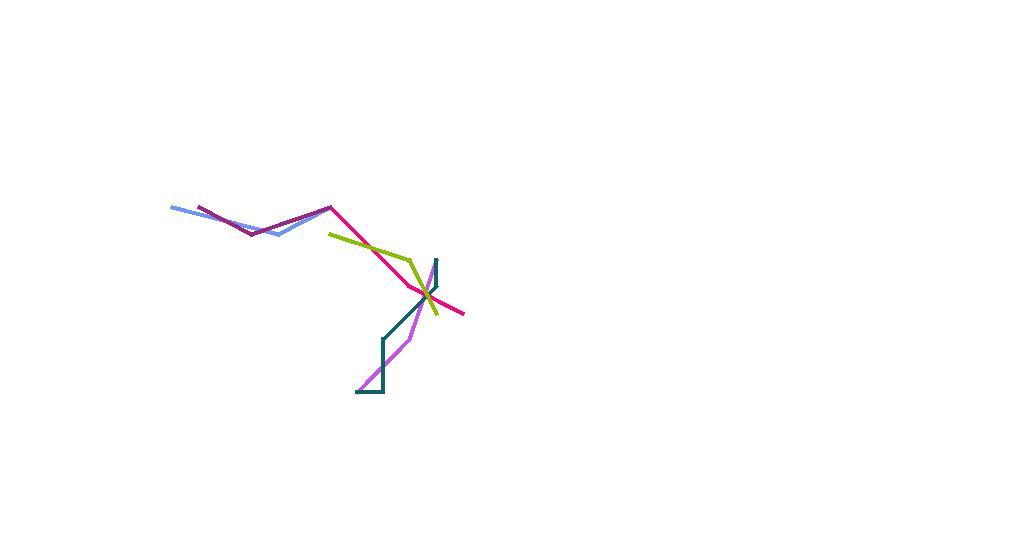
\includegraphics[width=0.85\linewidth]{1-6.png}}
% \end{figure*}
% 
% 
% \begin{figure*}[p]
% \fbox{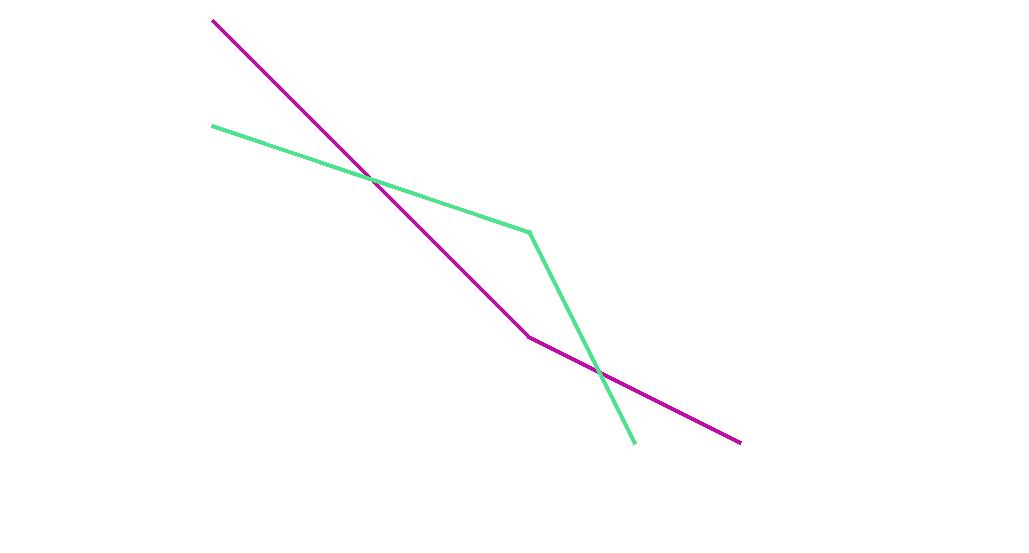
\includegraphics[width=0.65\linewidth]{3-4.png}}
% \end{figure*}
% 


% \section{User-interfaces}
% 
% 
% 
% 
% \framebox[4in][l]{\prompt \cmd{this is a command, short}}



\section{Download the program and a data set}
\index{download the program}

You must  download a binary for your plataform  of choice, to use \mt 


Linux version for 64 bits at \url{http://tux.uis.edu.co/labsist/pantrack/mt64.gz}

Linux version for 32 bits at \url{http://tux.uis.edu.co/labsist/pantrack/mt32.gz}
 

Windows version for 32, and 64 bits at \url{http://tux.uis.edu.co/labsist/pantrack/mt-win.zip}

and the data sets at \url{http://tux.uis.edu.co/labsist/pantrack/data-example.zip}


\vspace{-7\baselineskip}\footnotetext{For linux version you might need to convert the file \mt-xx to an execute file by typing in a command-line window:

 \framebox[2in][l] {\prompt \cmd{chmod +x \mt}}}
\vspace{7\baselineskip}


\section{Command modes}
\index{command modes}

PGTracks has two uses-interfaces: 1. A text user interface, and 2. a command-line interface. 


in the text user interface (TUI), the user can choice among different options including: changes of parameters for analysis, track a pair, groups or the whole data, find the index of congruence (IC) between pairs of tracks, or among sevaral tracks. print kml file, etc.
The command line interface was created for search strategies previously defined. The input file, output file and parameters files must be defined.

\vspace{-7\baselineskip}\footnotetext{\url{http://en.wikipedia.org/wiki/Text_user_interface\#TUI_under_Unix-like_systems}}
\vspace{7\baselineskip}

\subsection{Text user interface}

\index{tui:text user interface}

You can use the text interface by simply typing at the promt: 

\framebox[2in][l] {\prompt \cmd{ {\mt} }}

for Linux, and 

\framebox[2in][l] {\prompt \cmd{ {\mt -winXX.exe} }}

for Windows in a command-line window 


or by clicking on the PGTrack icon.

 
\vspace{-7\baselineskip}\footnotetext{
TUI typography: commands will be  \tui{c}ut, to indicate that the instruction is cut and the letter to be pressed is c]}
\vspace{7\baselineskip}


\textbf{1. Enter the input name}: As soon as you open PGTrack, it asks for the input file name:

\begin{center}
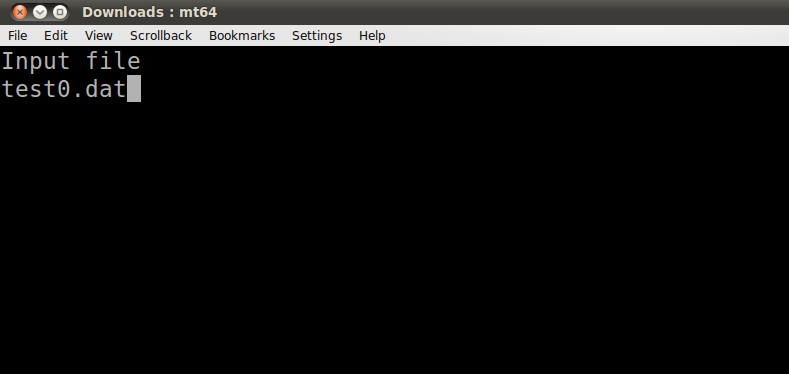
\includegraphics[scale=0.4]{./graphics/input-file.png}
 % input-file.png: 789x374 pixel, 72dpi, 27.83x13.19 cm, bb=0 0 789 374
\end{center}

\textbf{2. Set up the analysis:} Once you specified the input name, a list of commands help the users to set up the analysis.

\begin{center}
 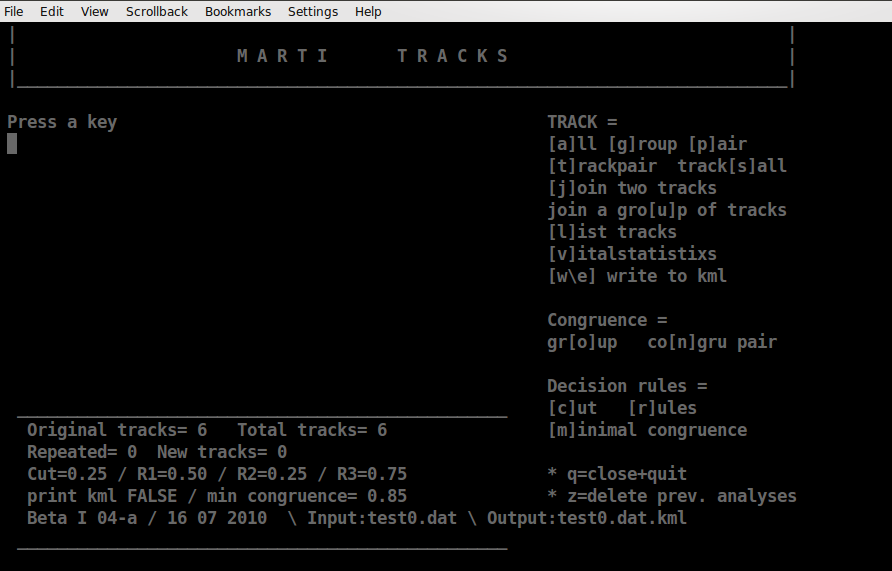
\includegraphics[scale=0.4]{./graphics/text-interface.png}
 % text-interface.png: 1237x678 pixel, 72dpi, 43.63x23.92 cm, bb=0 0 1237 678
\end{center}

First of all, we must define the values of the congruence parameters for the analysis. 

There are five parameters: \tui{c}ut value, 

three \tui{r}ules of decision R1, R2, R3, and a value for the \tui{m}inimal congruence.

For test0.dat we will use the following values:

\begin{center}
\begin{tabular}{ll}
\tui{c}ut & 0.25\\
\tui{r}ules & 0.75 0.5 1\\
\tui{m}inimal congruence & 0.8
\end{tabular}
\end{center}


\vspace{-7\baselineskip}\footnotetext{please remember:\\
to set each of these parameters you have to type the letters inside the square brackets [ ] and write the corresponding value foollowed by and enter}
\vspace{7\baselineskip}


\textbf{3. Search options}: Once the parameters have been defined, we will search the general patterns of distribution. 

First, s we might have similar initial MSTs, we need to find the similarity among the individual tracks to join a gro\tui{u}p of tracks according to the minimum value of \tui{m}inimal congruence fixed
 
In the case of test0.dat, we group from the track number 1 to the track number 6. Thus, we find if there are similar individual tracks that can be consider like the same track. 

Later, we need to redifined the values of the paramaters, in the case of test0.dat we will set:


\begin{center}
\begin{tabular}{ll}
\tui{c}ut & 0.5\\
\tui{r}ules & 1.5 1 2\\
\tui{m}inimal congruence & 0.8
\end{tabular}
\end{center}



Then, Typing \tui{a}ll, we will find the congruent segments for each individual tracks in order to delimitate the generalized tracks or distributional patterns of species.

Finally, we need to find the similarity among the generalized tracks, typing again \tui{u}, but joint from the track number 7 to the track 9, because first six track belong to the individual tracks.

\textbf{4. write a kml file }

Now, we need to write our results (the generalized tracks) in a kml file. For do that, first we must type \tui{k} to create a kml file, and [w] if we want to write the whole information of the analysis including: individual tracks, and generalized tracks, or we can type \tui{e} to write only the generalized tracks into the kml file.

\subsection{Command line interface}
\index{cli:ommand line interface}
For the command-line user interface we need to specified: the input file, output file, and parameters file.


For linux 64 bits:

\framebox[4.4in][l] {\prompt \cmd{ ./{\mt}-64 <input file> <output file> <parameters file>}}


For linux 32 bits:

\framebox[4.4in][l] {\prompt \cmd{ ./{\mt}-32 <input file> <output file> <parameters file>}}


For Windows 64 bits:

\framebox[4.5in][l] {\prompt \cmd{ {\mt}-64.exe <input file> <output file> <parameters file>}}


For Windows 64 bits:

\framebox[4.5in][l] {\prompt \cmd{ {\mt}-32.exe <input file> <output file> <parameters file>}}


\textbf{Output file:} it must have an extension .kml. 
\vspace{-7\baselineskip}\footnotetext{.kml file extension is mandatory with googleearth, otherwise googleearth will complain and will not open the file}
\vspace{7\baselineskip}


\textbf{parameters file:} This interface was designed for parameters/searching strategies defined previously. These search strategies have to be set in the parameters file. There are two main strategies, \pname{croizat0}, and \pname{croizat1}.

\vspace{-7\baselineskip}\footnotetext{
CL typography: commands will be  \pname{croizat0}, to indicate that the instruction is named Croizat0 and you must type \pname{croizat0} in your parameter file, the command could be written using lower or upper case.}
\vspace{7\baselineskip}




The framework of \pname{croizat0} is: 
\begin{enumerate}
 \item Find similar individual tracks by \tui{u} from the first, to the last individual tracks
 \item Calculate the congruent segments among individual tracks (delimitate generalized tracks) by \tui{a}
 \item Find similar generalized tracks by \tui{u} from the first, to the last generalized tracks
\end{enumerate}

The framework of \pname{croizat0} is: 
\begin{enumerate}
 \item Calculate the congruent segments among individual tracks (delimitate generalized tracks) by \tui{a}
 \item Find similar generalized tracks by \tui{u} from the first, to the last generalized tracks
\end{enumerate}

\textbf{Parameters} five values of the parameters could be defined: 


\begin{center}
\begin{tabular}{lll}
\tui{c}ut & &\pname{set cut <real value 0-360>} \\
\tui{r}ules & r1 & \pname{set lmax <real value 0-360>}\\
 & r2 & \pname{set lmin  <real value 0-360>}\\
 & r3 & \pname{set maxline  <real value 0-360>}\\
\tui{m}inimal congruence & & \pname{set ci <real value 0-1>}
\end{tabular}
\end{center}

\vspace{-7\baselineskip}\footnotetext{
cut value is a real <0 - 360> value expresed in degrees 0.0 = no cut - 360 = all points will be collapsed to one

minimal congruence is a real < 0-1> value. 0.0 = no congruence - 1.0 = totally congruent.

r1 to r3 is a real <0 - 360> value expresed in degrees

please refer to our paper (CITA) for further information}
\vspace{7\baselineskip}


These values  are used to calculate the similarity among individual tracks in all analyses joint or track


Thus, the commands for the analysis of test0.dat, using par1-search1.txt are:
\index{running test0.dat}

For linux 64 bits:

\framebox[4.4in][l] {\prompt \cmd{ ./{\mt}-64 test0.dat test0.kml par1-search1.txt}}


For linux 32 bits:

\framebox[4.4in][l] {\prompt \cmd{ ./{\mt}-32 test0.dat test0.kml par1-search1.txt}}


For Windows 64 bits:

\framebox[4.5in][l] {\prompt \cmd{ {\mt}-64.exe test0.dat test0.kml par1-search1.txt}}


For Windows 64 bits:

\framebox[4.5in][l] {\prompt \cmd{ {\mt}-32.exe test0.dat test0.kml par1-search1.txt}}



\subsection{Final results of test0.dat}


\begin{figure}[!ht]
\begin{center}
 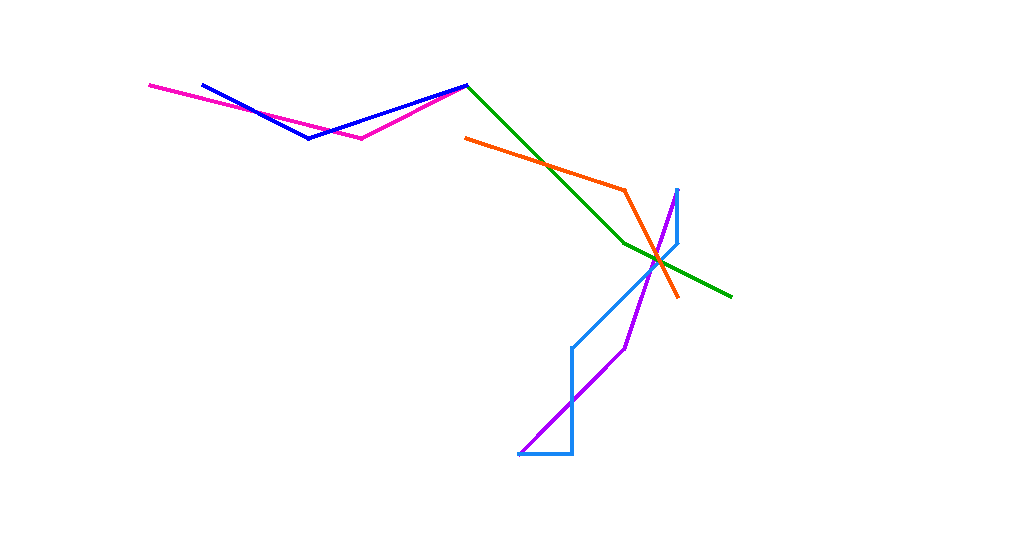
\includegraphics[scale=0.5]{./graphics/mst.png}
 % mst.png: 1029x553 pixel, 96dpi, 27.22x14.63 cm, bb=0 0 772 415
\end{center}
\caption{{\bf Individual tracks from test0.dat}}
\label{Figure1}
\end{figure}


\begin{figure}[!ht]
\begin{center}
 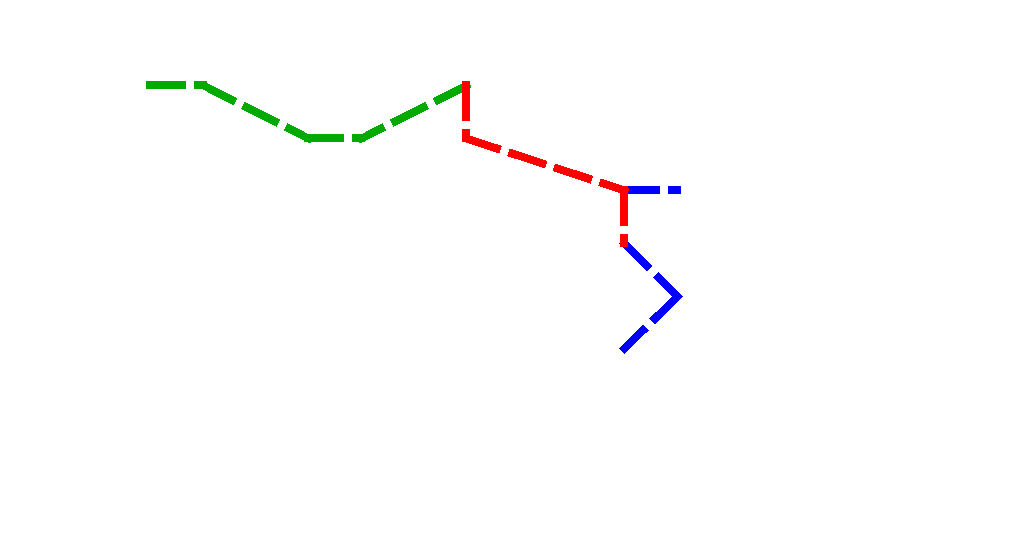
\includegraphics[scale=0.5]{./graphics/gtrack.png}
 % gtrack.png: 1029x553 pixel, 96dpi, 27.22x14.63 cm, bb=0 0 772 415
\end{center}
\caption{{\bf Generalized tracks from test0.dat}}
\label{Figure2}
\end{figure}

